\chapter{ADAPTER}

Il pattern Adapter è un design pattern strutturale che consente a due interfacce incompatibili di lavorare insieme, ovvero onsente a una classe di funzionare come 
un adattatore tra due interfacce incompatibili, consentendo loro di collaborare senza dover modificare il loro codice sorgente.

\section{Applicabilità}

Vogliamo usare una classe esistente ma la sua interfaccia non è compatibile con l'interfaccia che ci serve oppure vogliamo creare una classe riusabile che collaborerà 
con classi scorrelate.

\section{Struttura}

Abbiamo due varianti di questo pattern, una con ereditarietà ed una con object composition.

Nella prima variante abbiamo una classe, Adapter, che implementa l'interfaccia che ci serve, estendendo un'altra classe, Adaptee, cosicchè i metodi dell'interfaccia 
chiameranno i metodi di Adaptee.

\begin{figure}[H]
    \centering
    \includegraphics[width=0.5\linewidth]{../../immagini/adapter/struttura_adapter_ereditarietà}    
\end{figure}

Nella seconda variante, Adapter implementa l'interfaccia che ci serve delegando ad Adaptee e i metodi dell'interfaccia richiamano i metodi sull'oggetto Adaptee.

\begin{figure}[H]
    \centering
    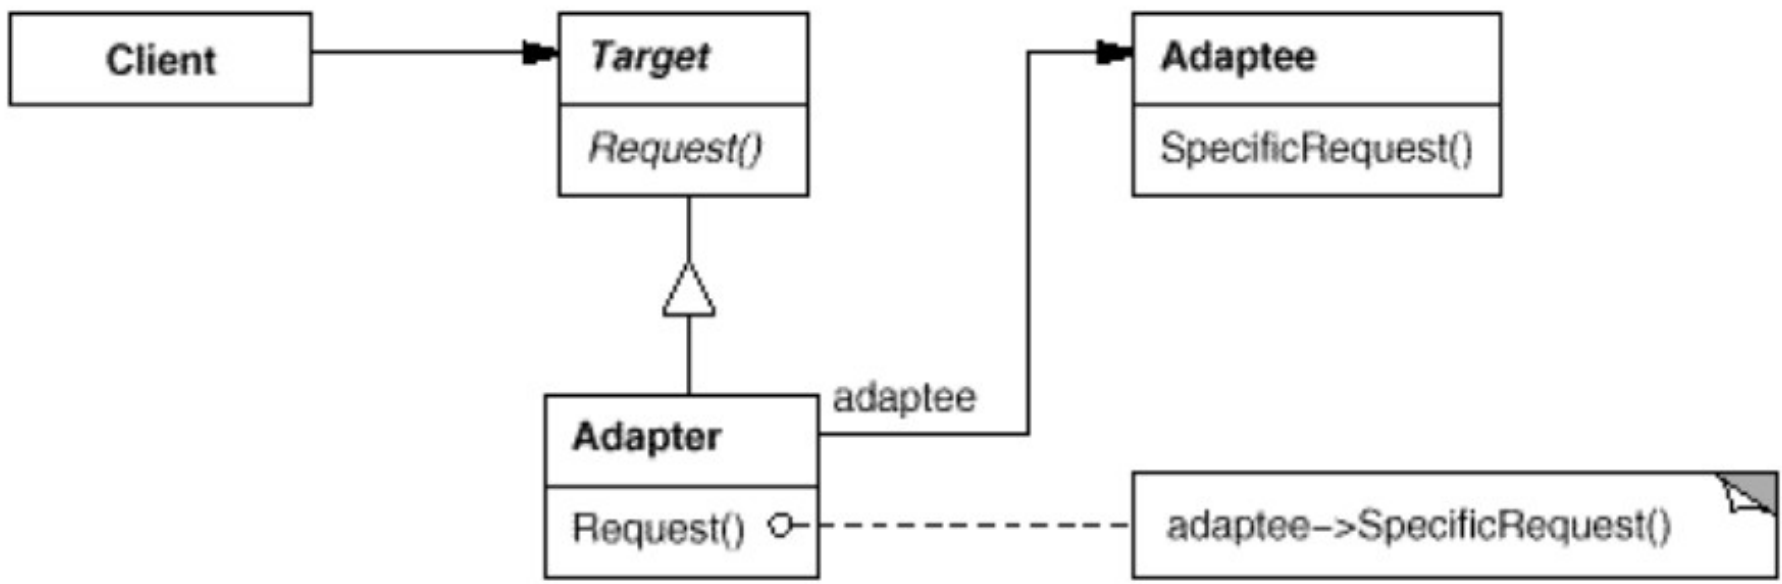
\includegraphics[width=0.5\linewidth]{../../immagini/adapter/struttura_adapter_composition}
\end{figure}

\textbf{Target} definisce l'interfaccia del dominio usata dai client;

\textbf{Client} collabora con gli oggetto conformi all'interfaccia Target;

\textbf{Adaptee} l'interfaccia esistente da adattare;

\textbf{Adapter} adatta l'interfaccia Adaptee a Target.

Client, a runtime, chiama operazioni su oggetto Adapter, staticamente di tipo Target, che a sua volta gestisce le operazioni chiamando in modo opportuno delle operazioni 
di Adaptee.

\section{Conseguenze}

Nella versione basata su ereditarietà, la classe Adapter adatta \textit{un certo tipo concreto} di Adaptee, quindi se volessi adattare un'altra classe concreta di 
Adaptee, allora dovremmo creare un nuovo adapter.

Possiamo ridefinire i metodi Adaptee in quanto è superclasse di Adapter.

Non introduciamo un nuovo livello di indirezione dovuto alla mancanza di object composition.

Nella versione basata su object composition, si può adattare \textit{qualsiasi} instanza di Adaptee, possiamo aggiugere del comportamento prima o dopo le operazioni di 
Adaptee ed introduciamo un ulteriore di livello di indirezione.

\medskip
\textbf{N.B.} In linguaggi tipo java, in cui ereditarietà implica subtyping, bisogna usare la versione object composition.

\section{Altro utilizzo di Adapter}

Esiste un altro caso d'uso di questo pattern.

Supponiamo di avere un'interfaccia con tanti metodi astratti che sono correlati tra loro (altrimenti si violerebbe ISP) e di avere una classe che la implementa.

Implementare un'interfaccia significa implementare tutti metodi dell'interfaccia anche se a noi iteresserebbero solo alcuni metodi.

Ecco che interviene l'Adapter, ovvero fa da ponte tra l'interfaccia, dando un'implementazione di default a tutti i metodi dell'interfaccia (tipicamente vuota), e la 
nostra classe, che estende Adapter e reimplementa solo i metodi che gli servono.

\medskip
\textbf{N.B.}L'implementazione di default si applica facilmente solo ai metodi void.

\section{Adapter vs default methods}

Questo pattern è un'alternativa ai default methods in quanto invece di stabilire una volta per tutte l'implementazione di default nell'interfaccia, non la tocchiamo e 
lasciamo più libertà allo sviluppatore.
